\documentclass[master=cws,masteroption=ai]{kulemt}
\setup{title={Algebraic Subtyping for Algebraic Types and Effects},
  author={Axel Faes},
  promotor={Prof.\,dr.\,ir.\ Tom Schrijvers},
  assessor={assesors},
  assistant={Amr Hany Saleh}}
% The following \setup may be removed entirely if no filing card is wanted
\setup{filingcard,
  translatedtitle=,
  udc=,
  shortabstract={}}

% Choose the main text font (e.g., Latin Modern)
\setup{font=lm}

%% Some recommended packages.
\usepackage{booktabs}   %% For formal tables:
                        %% http://ctan.org/pkg/booktabs
\usepackage{subcaption} %% For complex figures with subfigures/subcaptions
                        %% http://ctan.org/pkg/subcaption

\usepackage{array}
\usepackage{mathpartir}
\usepackage{xspace}
\usepackage{stmaryrd}
\usepackage{listings}
\usepackage{newtxmath}

%% Tikz Needed packages
\usepackage{pgfplots}
\pgfplotsset{width=7cm,compat=1.8}
\usepackage{pgfplotstable}
\renewcommand*{\familydefault}{\sfdefault}

% Finally the hyperref package is used for pdf files.
% This can be commented out for printed versions.
\usepackage[pdfusetitle,colorlinks,plainpages=false]{hyperref}

\newcommand{\lang}{\textsc{Effy}\xspace}
\newcommand{\eff}{\textsc{Eff}\xspace}
\newcommand{\core}{\textsc{EffCore}\xspace}
\newcommand{\ocaml}{\textsc{OCaml}\xspace}

% Meta-syntax
\newcommand{\bnfis}{\mathrel{\;{:}{:}\!=}\;}
\newcommand{\bnfor}{\mathrel{\;|\;}}
\newcommand{\defeq}{\mathrel{\;\stackrel{\text{def}}{=}\;}}
\newcommand{\set}[1]{\{ #1 \}}

% General syntactic constructs
\newcommand{\kord}[1]{\mathtt{#1}}
\newcommand{\kop}[1]{\;\mathtt{#1}\;}
\newcommand{\kpre}[1]{\mathtt{#1}\;}
\newcommand{\kpost}[1]{\;\mathtt{#1}}

% Types
\newcommand{\type}[1]{\mathtt{#1}}
\newcommand{\boolty}{\type{bool}}
\newcommand{\intty}{\type{int}}
\newcommand{\hto}{\Rightarrow}
\renewcommand{\C}{\underline{C}}
\newcommand{\D}{\underline{D}}
\newcommand{\dirt}{\Delta}
\newcommand{\dirtend}{. (\textsc{dot})}
\newcommand{\sig}{\Sigma}
\newcommand{\allops}{\Omega}

% Expressions and computations
\newcommand{\funtyped}[3]{\kpre{fun} #1 \T #2 \mapsto #3}
\newcommand{\rectype}[1]{\mu \alpha . #1}
\newcommand{\letvar}{\textbf{\^{x}}}
\newcommand{\union}{\sqcup}
\newcommand{\intersection}{\sqcap}
\newcommand{\emptyrow}{\emptyset}
\newcommand{\polytype}[1]{\forall \bar{\alpha} . #1}

\newcommand{\call}[3]{{{#1}\,{#2}\,{#3}}}
\newcommand{\case}{\mathop{\text{\texttt{|}}}}
\newcommand{\cont}[2]{(#1.\,#2)}
\newcommand{\const}{\kord{k}}
\newcommand{\fls}{\kord{false}}
\newcommand{\fun}[1]{\lambda #1 .} %\kpre{fun} #1 \mapsto}
\newcommand{\handler}[1]{\{ #1 \}}
\newcommand{\conditional}[3]{\kpre{if} #1 \kop{then} #2 \kop{else} #3}
\newcommand{\letin}[1]{\kpre{let} #1 \kop{in}}
\newcommand{\doin}[1]{\kpre{do} #1 \kop{ ; }}
\newcommand{\letrecin}[1]{\kpre{let} \kpre{rec} #1 \kop{in}}
\newcommand{\op}{\kord{Op}}
\newcommand{\ops}{\mathcal{O}}
\newcommand{\ocs}{\mathit{ocs}}
\newcommand{\ocsnil}{\kord{nil}}
\newcommand{\tru}{\kord{true}}
\newcommand{\ret}{\kpre{return}}
\newcommand{\withhandle}[2]{\kpre{handle} #2 \kop{with} #1}
\newcommand{\pure}[1]{\kord{pure } #1  }
\newcommand{\longcases}{\call{\op_1}{y}{k} \mapsto c_{\op_1}, \ldots, \call{\op_n}{x}{k} \mapsto c_{\op_n}}
\newcommand{\shortcases}{[\call{\op}{y}{k} \mapsto c_\op]_{\op \in \ops}}
\newcommand{\longhand}[1][\ret x \mapsto c_r]{\handler{#1, \longcases}}
\newcommand{\shorthand}[1][\ret x \mapsto c_r]{\handler{#1, \shortcases}}
\newcommand{\shorthandelab}[1][\ret x \mapsto c'_r]{\handler{#1, \shortcaseselab}}
\newcommand{\shortcaseselab}{[\call{\op}{y}{k} \mapsto c'_\op]_{\op \in \ops}}

% Type-checking
\newcommand{\row}{\mathrel{;} R}
\newcommand{\ctx}{\Gamma}
\newcommand{\ctxm}{\Xi}
\newcommand{\ctxp}{\Pi}
\newcommand{\ent}{\vdash}
\newcommand{\entt}{\Vdash}
\newcommand{\T}{\mathrel{:}}
\newcommand{\E}{\mathrel{!}}
\newcommand{\covers}{\mathrel{/}}
\renewcommand{\le}{\leqslant}

% Operational semantics
\newcommand{\eval}{\Downarrow}
\newcommand{\hs}{\mathcal{H}}
\newcommand{\nil}{\emptyset}
\newcommand{\cons}{\mathbin{::}}
\newcommand{\hseval}[1][\hs]{\Downarrow_{#1}}
\newcommand{\getval}[1]{{#1}_{\kord{val}}}
\newcommand{\getop}[1]{{#1}_{\kord{op}}}

\newcommand{\todo}[1]{\textcolor{red}{\textsc{Todo:} #1}}

% Needed to use the files from spec
\let\subparagraph\paragraph
\let\paragraph\subsubsection
\let\subsubsection\subsection
\let\subsection\section
\let\section\chapter

\begin{document}

\begin{preface}
  I would like to thank everybody who kept me busy the last year,
  especially my promoter and my assistants. I would also like to thank the
  jury for reading the text.
\end{preface}

\tableofcontents*

\begin{abstract}
  Algebraic effects and handlers are a very active area of research. An important aspect is the development of an optimising compiler. \eff is an ML-style language with support for effects and forms the testbed for the optimising compiler. However, the type-\&-effect system of \eff is unsatisfactory. This is due to the lack of some elegant properties. It is also awkward to implement and use in practice.
\end{abstract}

\listoffigures
\listoftables

% Now comes the main text
\mainmatter

\section{Introduction}
The specification for a type-\&-effect system with algebraic subtyping for algebraic effects and handlers is given in this document. The formal properties of this system are studied in order to find which properties are satisfied compared to other type-\&-effect systems. The proposed type-\&-effect system builds on two very recent developments in the area of programming language theory.

\paragraph{Algebraic subtyping}
In his December 2016 PhD thesis, Stephen Dolan (University of Cambridge, UK), has presented a novel type system that combines subtyping and parametric polymorphism in a particulary attractive and elegant fashion. A cornerstone of his design are the algebraic properties that the subtyping relation should respect.

\paragraph{Algebraic effects and handlers}
These are a new formalism for formally modelling side-effects (e.g. mutable state or non-determinism) in programming languages, developed by Matija Pretnar (University of Ljubjana) and Gordon Plotkin (University of Edinburgh). This approach is gaining a lot of traction, not only as a formalism but also as a practical feature in actual programming languages (e.g. the Koka language developed by Microsoft Research). We are collaborating with Matija Pretnar on the efficient implementation of one such language, called Eff. Axel Faes has contributed to this collaboration during a project he did for the Honoursprogramme of the Faculty of Engineering Science.

\subsection{Motivation}
Algebraic effects and handlers benefit from a custom type-\&-effect system, a type system that also tracks which effects can happen in a program. Several such type-\&-effect systems have been proposed in the literature, but all are unsatisfactory. We attribute this to the lack of the elegant properties of Dolan's type system. Indeed the existing type-\&-effect systems are not only theoretically unsatisfactory, but they are also awkward to implement and use in practice.

\paragraph{Research questions}
\begin{itemize}
\item How can Dolan's elegant type system be extended with effect information?
\item Which properties are preserved and which aren't preserved?
\item What advantages are there to an type-\&-effect system based on Dolan's elegant type system?
\end{itemize}

\subsection{Goals}
The goal of this thesis is to derive a type-\&-effect system that extends Dolan's elegant type system with effect information. This type-\&-effect system should inherit Dolan's harmonious combination of subtyping (in our case induced by a lattice structure on the effect information) with parametric polymorphism and preserve all of its desirable properties (both low-level algebraic properties and high-level meta-theoretical properties like type soundness and the existence of principal types). Afterwards this type-\&-effect system The following approach is taken:
\begin{enumerate}
\item Study of the relevant literature and theoretical background.
\item Design of a type-\&-effect system derived from Dolan's, that integrates effects.
\item Proving the desirable properties of the proposed type-\&-effect system: type soundness, principal typing, ...
\item Time permitting: Design of a type inference algorithm that derives the principal types of programs without type annotations and proving its correctness.
\item Time permitting: Implementation of the algorithm and comparing it to other algorithms (such as row polymorphism based type-\&-effect systems).
\end{enumerate}

\subsection{Results}
Describe what the resulting product is and how it is useful or provides an advantage over other solutions.

\section{Background}
In this section, I will provide the background necessary to be able to read the text. This includes an introduction into programming languages (and programming language theory) and algebraic effect handlers 

Dolan's type system and \eff are discussed in further chapters and thus shouldn't need to be explained in this section.

\section{Related Work (Algebraic Subtyping)}
Subtyping is a partial order which is a reflexive transitive binary relation satisfying antisymmetry (subtyping rules). The subtyping order also forms a distributive lattice (equivalence rules). 



\section{Related Work (\eff)}
The type-\&-effect system that is used in \eff is based on subtyping and dirty types \cite{effectsystem}.

\subsection{Types and terms}

\paragraph{Terms}
Figure~\ref{fig:terms:eff} shows the two types of terms in \eff. There are values $v$ and computations $c$. Computations are terms that can contain effects. Effects are denoted as operations $Op$ which can be called.

\begin{figure}[!htb]
\begin{center}
\framebox{
\begin{minipage}{0.98\columnwidth}
\[\begin{array}{r@{~}c@{~}l@{\quad}l}
  \text{value}~v & \bnfis {} & x & \text{variable} \\ %\lambda\text{-variable} \\
    % & \bnfor & \letvar & \text{let-variable} \\
    % & \bnfor & \const & \text{constant} \\
    & \bnfor & \tru & \text{true} \\
    & \bnfor & \fls & \text{false} \\
    & \bnfor & \fun{x} c & \text{function} \\
    & \bnfor & \{ & \text{handler} \\
    & & \quad \ret x \mapsto c_r, & \quad\text{return case} \\
    & & \quad \shortcases & \quad\text{operation cases} \\
    & & \} & \\
  \text{comp}~c & \bnfis & v_1 \, v_2 & \text{application} \\
    & \bnfor & \doin{x \leftarrow c_1} c_2 & \text{sequencing} \\
    & \bnfor & \conditional{e}{c_1}{c_2} & \text{conditional} \\
    & \bnfor & \letrecin{f \, x = c_1} c_2 & \text{rec definition} \\
    & \bnfor & \ret v  & \text{returned val} \\
    & \bnfor & \op \, v & \text{operation call} \\
    & \bnfor & \withhandle{v}{c} & \text{handling}
\end{array}\]
\end{minipage}
}
\end{center}
\caption{Terms of \eff}\label{fig:terms:eff}
\end{figure}

\paragraph{Types}
Figure~\ref{fig:types:eff} shows the types of \eff. There are two main sorts of types. There are (pure) types $A, B$ and dirty types $\C, \D$. A dirty type is a pure type $A$ tagged with a finite set of operations $\dirt$, which we call dirt, that can be called. This finite set $\dirt$ is an over-approximation of the operations that are actually called. The type $\C \hto \D$ is used for handlers because a handler takes an input computation $\C$, handles the effects in this computation and outputs computation $\D$ as the result.

\begin{figure}[!htb]
\begin{center}
\framebox{
\begin{minipage}{0.98\columnwidth}
\[\begin{array}{r@{~}c@{~}l@{\quad}l}
  \text{(pure) type}~A, B & \bnfis {}
    % & \boolty \bnfor \intty & \text{basic types} \\
    & \boolty & \text{bool type} \\
    & \bnfor & A \to \C & \text{function type} \\
    & \bnfor & \C \hto \D & \text{handler type} \\
  \text{dirty type}~\C, \D & \bnfis {} & A \E \dirt \\
  \text{dirt}~\dirt & \bnfis {} &\set{\op_1, \dots, \op_n}
\end{array}\]
\end{minipage}
}
\end{center}
\caption{Types of \eff}\label{fig:types:eff}
\end{figure}

\subsection{Subtyping}
\eff uses a subtyping based system. Subtyping is a form of type polymorphism. Types can be related to eachother, being either subtypes or supertypes. Intuitively one could think about Java classes and inheritance in order to understand subtyping. There are some big differences between inheritance and subtyping, but from the principle of gaining an understanding of what subtyping entails, the relation between the two can be made. 

Let us take the subtyping judgement $\boolty \le \boolty$. This judgement is about reflexivity. It states that $\boolty$ is a subtype of itself. The subtyping judgement for the arrow type (functions) states that, if we have $A' \le A$ and $\C \le \C'$, then we also induce the natural subtyping judgement $A \to \C \le A' \to \C'$. This tells us that, if we have a function, the caller can always call that function with a type that is "more" and that function can always return "more" than what the caller expects. This can be easily visualised when the argument and return values are records. If a function requires a record with labels "x" and "y", the caller is allowed to call the function with a record containing more that just "x" and "y". A similar analogy can be made for the return values. Functions are contravariant in its argument types and covariant in its return types.

The dirty type $A \E \dirt$ is assigned to a computation returning values of type $A$ and potentially calling operations from the set $\dirt$. This set $\dirt$ is always an over-approximation of the actually called operations, and may safely be increased, inducing a natural subtyping judgement $A \E \dirt \le A \E \dirt'$ on dirty types where $\dirt'$ contains extra operations compared to $\dirt$. As dirty types can occur inside pure types, we also get a derived subtyping judgement on pure types. Both judgements are defined in Figure~\ref{fig:subtyping}. Observe that, as usual, subtyping is contravariant in the argument types of functions as well as handlers, and covariant in their return types. \cite{inferring}

\begin{figure}[!htb]
\begin{center}
\framebox{
\begin{minipage}{0.95\columnwidth}
\textbf{Subtyping}
\begin{mathpar}
  \inferrule[Sub-$\boolty$]{
  }{
    \boolty \le \boolty
  }

  \inferrule[Sub-$\to$]{
    A' \le A \\
    \C \le \C'
  }{
    A \to \C \le A' \to \C'
  }

  \inferrule[Sub-$\hto$]{
    \C' \le \C \\
    \D \le \D'
  }{
    \C \hto \D \le \C' \hto \D'
  }

  \inferrule[Sub-$\E$]{
    A \le A' \\
    \dirt \subseteq \dirt'
  }{
    A \E \dirt \le A' \E \dirt'
  }
\end{mathpar}
\end{minipage}
}
\end{center}
\caption{Subtyping for pure and dirty types of \eff}\label{fig:subtyping}
\end{figure}

\subsection{Typing rules}
Figure~\ref{fig:eff-typing:e} and figure~\ref{fig:eff-typing:c} defines the typing judgements for values and computations with respect to a standard typing context $\ctx$. This types context can contain $\epsilon$ or a variable with a type.

\paragraph{Values}
The rules for subtyping, variables, and functions are entirely standard.

A handler expression has type $A \E \dirt \cup \ops \hto B \E \dirt$ iff all branches (both the operation cases and the return case) have dirty type $B \E \dirt$ and the operation cases cover the set of operations $\ops$. Note that the intersection $\dirt \cap \ops$ is not necessarily empty. The handler deals with the operations $\ops$, but in the process may re-issue some of them (i.e., $\dirt \cap \ops$).

When typing operation cases, the given signature for the operation $(\op \T A_\op \to B_\op) \in \sig$ determines the type $A_\op$ of the parameter $x$ and the domain $B_\op$ of the continuation $k$. As our handlers are deep, the codomain of $k$ should be the same as the type $B \E \dirt$ of the cases. \cite{inferring}

\paragraph{Computations}
With the following exceptions, the typing judgement $\ctx \ent c : \C$ has a straightforward definition. The $\ret$ construct renders a value $v$ as a pure computation, i.e., with empty dirt. An operation invocation $\op\,v$ is typed according to the operation's signature, with the operation itself as its only operation. Finally, rule \textsc{With} shows that a handler with type $\C \hto \D$ transforms a computation with type $\C$ into a computation with type $\D$. \cite{inferring}

\begin{figure}[H]
\begin{center}
\framebox{
\begin{minipage}{0.95\columnwidth}
\[\begin{array}{r@{~}c@{~}l}
  \text{typing contexts}~\ctx & \bnfis {} & \epsilon \bnfor \ctx, x : A\\
\end{array}\]
\textbf{Expressions}
\begin{mathpar}
  \inferrule[SubVal]{
    \ctx \ent v \T A \\
    A \le A'
  }{
    \ctx \ent v \T A'
  }

  \inferrule[Var]{
    (x \T A) \in \ctx
  }{
    \ctx \ent x \T A
  }

  % \inferrule[Const]{
  %   (\const \T A) \in \sig
  % }{
  %   \ctx \ent \const \T A
  % }

  \inferrule[True]{
  }{
    \ctx \ent \tru \T bool
  }

  \inferrule[False]{
  }{
    \ctx \ent \fls \T bool
  }
  
  \inferrule[Fun]{
    \ctx, x \T A \ent c \T \C
  }{
    \ctx \ent \fun{x} c \T A \to \C
  }

  \inferrule[Hand]{
    \ctx, x \T A \ent c_r \T B \E \dirt \\
    \Big[
      (\op \T A_\op \to B_\op) \in \sig \qquad \\
      \ctx, y \T A_\op, k \T B_\op \to B \E \dirt \ent c_\op \T B \E \dirt
    \Big]_{\op \in \ops}
  }{
    \ctx \ent \shorthand \T \\ A \E \dirt \cup \ops \hto B \E \dirt
  }
\end{mathpar}
\end{minipage}
}
\end{center}
\caption{Typing of expressions in \eff}\label{fig:eff-typing:e}
\end{figure}

\begin{figure}[H]
  \begin{center}
  \framebox{
  \begin{minipage}{0.95\columnwidth}
  \[\begin{array}{r@{~}c@{~}l}
    \text{typing contexts}~\ctx & \bnfis {} & \epsilon \bnfor \ctx, x : A\\
  \end{array}\]
\textbf{Computations}
\begin{mathpar}
  \inferrule[SubComp]{
    \ctx \ent c \T \C \\
    \C \le \C'
  }{
    \ctx \ent c \T \C'
  }

  \inferrule[App]{
    \ctx \ent v_1 \T A \to \C \\
    \ctx \ent v_2 \T A
  }{
    \ctx \ent v_1 \, v_2 \T \C
  }

  \inferrule[Cond]{
    \ctx \ent v \T bool \\
    \ctx \ent c_1 \T \C \\
    \ctx \ent c_2 \T \C \\
  }{
    \ctx \ent \conditional{v}{c_1}{c_2} \T \C
  }

  \inferrule[LetRec]{
    \ctx, f \T A \to \C, x \T A \ent c_1 \T \C \\
    \ctx, f \T A \to \C \ent c_2 \T \D
  }{
    \ctx \ent \letrecin{f \, x = c_1} c_2 \T \D
  }

  \inferrule[Ret]{
    \ctx \ent v \T A
  }{
    \ctx \ent \ret v \T A \E \emptyset
  }

  \inferrule[Op]{
    (\op \T A \to B) \in \sig \\
    \ctx \ent v \T A
  }{
    \ctx \ent \op \, v \T B \E \{\op\}
  }

  \inferrule[Do]{
    \ctx \ent c_1 \T A \E \dirt \\
    \ctx, x \T A \ent c_2 \T B \E \dirt
  }{
    \ctx \ent \doin{x \leftarrow c_1} c_2 \T B \E \dirt
  }

  \inferrule[With]{
    \ctx \ent v \T \C \hto \D \\
    \ctx \ent c \T \C
  }{
    \ctx \ent \withhandle{v}{c} \T \D
  }
\end{mathpar}
\end{minipage}
}
\end{center}
\caption{Typing of computations in \eff}\label{fig:eff-typing:c}
\end{figure}

\subsection{Type Inference}\label{type-inference-explain}
Type inference is the process where types are automatically inferred by the compiler. Types rules are used as a blueprint for type inference. Every typing rule indicates a situation a program can be in at any point in time. Thus, for every typing rule, there has to be a type inference rule. 

In the case of a subtyping based system, contraint-based type inference rules are used. The specific rules for \eff are not fully given as they are not required for the work in this thesis. The idea behind constraint-based type inference rules is that, in each rule, constraints can be made. In case of a subtyping based system, these constraints are subtyping constraints between two types. 

In figure~\ref{fig:inference:eff}, the type inference for function specialization can be seen. We have two expressions $v_1$ and $v_2$ with types $A_1$ and $A_2$. The application produces some type $\alpha \E \delta$. In order to link the types of the two expressions to the produced type, a subtyping constraint is used. The constraint $A_1 \le A_2 \to (\alpha \E \delta)$ indicates that $A_1$ has to be a subtype of a function type $A_2 \to (\alpha \E \delta)$. 

The reader may wonder what happens when the subtyping constraint is changed into an equality constraint $A_1 = A_2 \to (\alpha \E \delta)$. If every subtyping relation is changed into an equality relation, including for all relations in the subtyping rules in figure~\ref{fig:subtyping}, than we have changed the subtyping system into a Hindley-Milner system. The Hindley-Milner system is less expressive than the subtyping system. This makes sense as an equation with subtyping $\le$ allows for more solutions than using equality $=$.

For every typing rule, there is a type inference rule. At the end of the of applying all the rules, $\ctrs$ contains a lot of constraints. These constraints are solved as much as possible using substitution techniques. Subtyping does not allow for all constraints to be completely solved. In contrast, the Hindley-Milner system can solve all constraints with substitution techniques.

\begin{figure}[H]
\begin{center}
  \begin{framed}
  \begin{minipage}[t]{0.95\columnwidth}
  \[\begin{array}{r@{~}c@{~}l}
      \text{typing contexts}~\ctx & \bnfis {} & \epsilon \bnfor \ctx, x : A\\
      \end{array}\]
  \textbf{Computations}
      \begin{mathpar}
      \inferrule[App]{
          \ctx \prinent v_1 \T A_1 \\
          \ctx \prinent v_2 \T A_2
      }{
          \ctx \prinent v_1 \, v_2 \T \alpha \E \delta
      } \ctrs = \ctrs \cup (A_1 \le A_2 \to (\alpha \E \delta))
      \end{mathpar}
  \end{minipage}
  \end{framed}
  \end{center}
  \caption{Type inference rule for function application for \eff}\label{fig:inference:eff}
  \end{figure}
  

\section{Core Language (\core)}

\core is a language with row-based effects, intersection and union types and effects and is subtyping based. 

Define your problem very clearly. Provide a formal definition if possible, using mathematical definitions.

\subsection{Types and terms}

\paragraph{Terms}
Figure~\ref{fig:terms:core} shows the two types of terms in \core. Just like in \eff. there are values $v$ and computations $c$. Computations are terms that can contain effects. Effects are denoted as operations $Op$ which can be called. The only change compared to \eff is that \core makes a distinction between let-bound variables and lambda-bound variables. This distinction was introduced by Dolan in order to simplify the algebraic subtyping approach \cite{mlsub}. By making this distinction, a distinction can be made between monomorphic variables (lambda-bound) and polymorphic variables (let-bound) at the term level.

\begin{figure}[!htb]
\begin{center}
\framebox{
\begin{minipage}{0.98\columnwidth}
\[\begin{array}{r@{~}c@{~}l@{\quad}l}
  \text{value}~v & \bnfis {} & x & \lambda\text{-variable} \\
    & \bnfor & \letvar & \text{let-variable} \\
    & \bnfor & \tru & \text{true} \\
    & \bnfor & \fls & \text{false} \\
    & \bnfor & \fun{x}c & \text{function} \\
    & \bnfor & \{ & \text{handler} \\
    & & \quad \ret x \mapsto c_r, & \quad\text{return case} \\
    & & \quad \shortcases & \quad\text{operation cases} \\
    & & \} & \\
  \text{comp}~c & \bnfis & v_1 \, v_2 & \text{application} \\
    & \bnfor & \doin{\letvar = c_1} c_2 & \text{sequencing} \\
    & \bnfor & \letin{\letvar = v} c & \text{let} \\
    & \bnfor & \conditional{e}{c_1}{c_2} & \text{conditional} \\
    & \bnfor & \ret v  & \text{returned val} \\
    & \bnfor & \op \, v & \text{operation call} \\
    & \bnfor & \withhandle{v}{c} & \text{handling}
\end{array}\]
\end{minipage}
}
\end{center}
\caption{Terms of \core}\label{fig:terms:core}
\end{figure}

\paragraph{Types}
Figure~\ref{fig:types:core} shows the types of \core. There are, like in \eff, two main sorts of types. There are (pure) types $A, B$ and dirty types $\C, \D$. A dirty type is a pure type $A$ tagged with a finite set of operations $\dirt$, which we call dirt, that can be called. It can also be an union or intersection of dirty types. In further sections, the relations between dirty intersections or unions and pure intersections or unions are explained. The finite set $\dirt$ is an over-approximation of the operations that are actually called. Row variables are introduced as well as intersection and unions. The $\dirtend$ is used to close rows that do not end with a row variable. The type $\C \hto \D$ is used for handlers because a handler takes an input computation $\C$, handles the effects in this computation and outputs computation $\D$ as the result. \cite{handling}

However, now the effects of the algebraic subtyping approach become apparant. Different types are added in order to support the subtyping. These are a type variables, recursive type, top, bottom, intersection and union \cite{mlsub}. The novel element here is the combination of the algebraic effects and algebraic subtyping. There needs to be a way to bring the dirts into the algebraic subtyping framework. Since the recursive element is handled at the term level, there is no need for recursive dirts. Aside from this and the lack of a function and handler type, the dirts mirror the types.

\begin{figure}[!htb]
\begin{center}
\framebox{
\begin{minipage}{0.98\columnwidth}
\[\begin{array}{r@{~}c@{~}l@{\quad}l}
  \text{typing contexts}~\ctx & \bnfis {} & \epsilon \bnfor \ctx, x : A \bnfor \ctx, \letvar : \polytype{B}\\
  \text{monomorphic typing contexts}~\ctxm & \bnfis {} & \epsilon \bnfor \ctxm, x : A\\
  \text{polymorphic typing contexts}~\ctxp & \bnfis {} & \epsilon \bnfor \ctxp, \letvar : [\ctxm]A\\
  \text{(pure) type}~A, B & \bnfis {}
    & \boolty & \text{bool type} \\
    & \bnfor & A \to \C & \text{function type} \\
    & \bnfor & \C \hto \D & \text{handler type} \\
    & \bnfor & \alpha & \text{type variable} \\
    & \bnfor & \rectype{A} & \text{recursive type} \\
    & \bnfor & \top & \text{top} \\
    & \bnfor & \bot & \text{bottom} \\
    & \bnfor & A \intersection B & \text{intersection} \\
    & \bnfor & A \union B & \text{union} \\
  \text{dirty type}~\C, \D & \bnfis {} & A \E \dirt \\
    
  \text{dirt}~\dirt & \bnfis {} & \op & \text{operation} \\
    & \bnfor & \delta & \text{dirt variable} \\
    & \bnfor & \emptyrow & \text{empty dirt} \\
    & \bnfor & \dirt_1 \intersection \dirt_2 & \text{intersection} \\
    & \bnfor & \dirt_1 \union \dirt_2 & \text{union} \\
  \text{All operations}~\allops & \bnfis {} & \bigsqcup \op_i | \op_i \in \sig \\
\end{array}\]
\end{minipage}
}
\end{center}
\caption{Types of \core}\label{fig:types:core}
\end{figure}

\subsection{Type system}

\todo{explain equivalance rules}

\begin{figure}[!htb]
\begin{center}
\begin{framed}
\begin{minipage}[t]{0.95\columnwidth}
\begin{mathpar}    
    \inferrule[]{}{
        A_1 \le A_2 \leftrightarrow A_1 \union A_2 \equiv A_2
    }\\

    \inferrule[]{}{
        A_1 \le A_2 \leftrightarrow A_1 \equiv A_1 \intersection A_2
    }\\

    % \inferrule[]{}{
    %     \op \le \delta_1 \leftrightarrow \delta_2 = \op \union \delta_1, \op \union \delta_2 \equiv \delta_2
    % }\\

    \inferrule[]{}{
        \dirt_1 \le \dirt_2 \leftrightarrow \dirt_1 \union \dirt_2 \equiv \dirt_2
    }\\

    \inferrule[]{}{
        \dirt_1 \le \dirt_2 \leftrightarrow \dirt_1 \equiv \dirt_1 \intersection \dirt_2
    }\\

    \inferrule[]{}{
        \C_1 \le \C_2 \leftrightarrow \C_1 \union \C_2 \equiv \C_2
    }\\

    \inferrule[]{}{
        \C_1 \le \C_2 \leftrightarrow \C_1 \equiv \C_1 \intersection \C_2
    }
\end{mathpar}
\end{minipage}
\end{framed}
\end{center}
\caption{Relationship between Equivalence and Subtyping}\label{fig:core-relation}
\end{figure}


\begin{figure}[!htb]
\begin{center}
\begin{framed}
% \framebox{
\begin{minipage}[t]{0.475\columnwidth}
% \textbf{Equations of distributive lattices for types}
\begin{mathpar}
    \inferrule[]{}{
      A \union A \equiv A
    }\\
    
    \inferrule[]{}{
      A_1 \union A_2 \equiv A_2 \union A_1
    }\\

    \inferrule[]{}{
      A_1 \union (A_2 \union A_3) \equiv (A_1 \union A_2) \union A_3
    }\\

    \inferrule[]{}{
      A_1 \union (A_1 \intersection A_2) \equiv A_1
    }\\

    \inferrule[]{}{
      \bot \union A \equiv A
    }\\

    \inferrule[]{}{
      \top \union A \equiv \top
    }
\end{mathpar}
\end{minipage}
\begin{minipage}[t]{0.475\columnwidth}
\begin{mathpar}    
    \inferrule[]{}{
        A \intersection A \equiv A
    }\\

    \inferrule[]{}{
        A_1 \intersection A_2 \equiv A_2 \intersection A_1
    }\\

    \inferrule[]{}{
        A_1 \intersection (A_2 \intersection A_3) \equiv (A_1 \intersection A_2) \intersection A_3
    }\\

    \inferrule[]{}{
        A_1 \intersection (A_1 \union A_2) \equiv A_1
    }\\

    \inferrule[]{}{
        \bot \intersection A \equiv \bot
    }\\

    \inferrule[]{}{
        \top \intersection A \equiv A
    }
\end{mathpar}
\end{minipage}
\begin{minipage}[t]{0.95\columnwidth}
\begin{mathpar}    
    \inferrule[]{}{
        A_1 \union (A_2 \intersection A_3) \equiv (A_1 \union A_2) \intersection (A_1 \union A_3)
    }\\

    \inferrule[]{}{
        A_1 \intersection (A_2 \union A_3) \equiv (A_1 \intersection A_2) \union (A_1 \intersection A_3)
    }
\end{mathpar}
\end{minipage}
% }
\end{framed}
\end{center}
\caption{Equations of distributive lattices for types}\label{fig:core-equations-types}
\end{figure}

\begin{figure}[!htb]
\begin{center}
\begin{framed}
\begin{minipage}[t]{0.95\columnwidth}
\begin{mathpar}    
    \inferrule[]{}{
        (A_1 \to \C_1) \union (A_2 \to \C_2) \equiv (A_1 \intersection A_2) \to (\C_1 \union \C_2)
    }\\

    \inferrule[]{}{
        (A_1 \to \C_1) \intersection (A_2 \to \C_2) \equiv (A_1 \union A_2) \to (\C_1 \intersection \C_2)
    }\\

    \inferrule[]{}{
        (A_1 \hto \C_1) \union (A_2 \hto \C_2) \equiv (A_1 \intersection A_2) \hto (\C_1 \union \C_2)
    }\\

    \inferrule[]{}{
        (A_1 \hto \C_1) \intersection (A_2 \hto \C_2) \equiv (A_1 \union A_2) \hto (\C_1 \intersection \C_2)
    }\\
    
    \inferrule[]{}{
        (\C_1 \union \C_2) \equiv (A_1 \E \dirt_1 \union A_2 \E \dirt_2) \equiv (A_1 \union A_2) \E (\dirt_1 \union \dirt_2)
    }\\

    \inferrule[]{}{
        (\C_1 \intersection \C_2) \equiv (A_1 \E \dirt_1 \intersection A_2 \E \dirt_2) \equiv (A_1 \intersection A_2) \E (\dirt_1 \intersection \dirt_2)
    }
\end{mathpar}
\end{minipage}
\end{framed}
\end{center}
\caption{Equations for function, handler and dirty types}\label{fig:core-equations-other-types}
\end{figure}

\begin{figure}[!htb]
\begin{center}
\begin{framed}
% \framebox{
\begin{minipage}[t]{0.475\columnwidth}
\begin{mathpar}
    \inferrule[]{}{
        \dirt \union \dirt \equiv \dirt
    }\\
    
    \inferrule[]{}{
        \dirt_1 \union \dirt_2 \equiv \dirt_2 \union \dirt_1
    }\\

    \inferrule[]{}{
        \dirt_1 \union (\dirt_2 \union \dirt_3) \equiv (\dirt_1 \union \dirt_2) \union \dirt_3
    }\\

    \inferrule[]{}{
        \dirt_1 \union (\dirt_1 \intersection \dirt_2) \equiv \dirt_1
    }\\

    \inferrule[]{}{
        \emptyrow \union \dirt \equiv \dirt
    }\\

    \inferrule[]{}{
        \allops \union \dirt \equiv \allops
    }
\end{mathpar}
\end{minipage}
\begin{minipage}[t]{0.475\columnwidth}
\begin{mathpar}    
    \inferrule[]{}{
        \dirt \intersection \dirt \equiv \dirt
    }\\

    \inferrule[]{}{
        \dirt_1 \intersection \dirt_2 \equiv \dirt_2 \intersection \dirt_1
    }\\

    \inferrule[]{}{
        \dirt_1 \intersection (\dirt_2 \intersection \dirt_3) \equiv (\dirt_1 \intersection \dirt_2) \intersection \dirt_3
    }\\

    \inferrule[]{}{
        \dirt_1 \intersection (\dirt_1 \union \dirt_2) \equiv \dirt_1
    }\\

    \inferrule[]{}{
        \emptyrow \intersection \dirt \equiv \emptyrow
    }\\

    \inferrule[]{}{
        \allops \intersection \dirt \equiv \dirt
    }
\end{mathpar}
\end{minipage}
\begin{minipage}[t]{0.95\columnwidth}
\begin{mathpar}    
    \inferrule[]{}{
        \dirt_1 \union (\dirt_2 \intersection \dirt_3) \equiv (\dirt_1 \union \dirt_2) \intersection (\dirt_1 \union \dirt_3)
    }\\

    \inferrule[]{}{
        \dirt_1 \intersection (\dirt_2 \union \dirt_3) \equiv (\dirt_1 \intersection \dirt_2) \union (\dirt_1 \intersection \dirt_3)
    }
\end{mathpar}
\end{minipage}
% }
\end{framed}
\end{center}
\caption{Equations of distributive lattices for dirts}\label{fig:core-equations-dirts}
\end{figure}
% \subsection{Subtyping rules}
% The subtyping rules are given in Figure~\ref{fig:core-subtyping} and Figure~\ref{fig:core-subtyping-dirt}. Figure~\ref{fig:core-subtyping} contains all subtyping rules related to types. Figure~\ref{fig:core-subtyping-dirt} contains the subtyping rules that govern the dirts.

% The dirty type $A \E \dirt$ is assigned to a computation returning values of type $A$ and potentially calling operations from the set $\dirt$. This set $\dirt$ is always an over-approximation of the actually called operations, and may safely be increased, inducing a natural subtyping judgement $A \E \dirt \leq A \E \dirt'$ on dirty types. As dirty types can occur inside pure types, we also get a derived subtyping judgement on pure types. Observe that, as usual, subtyping is contravariant in the argument types of functions and handlers, and covariant in their return types.

% \paragraph{Dirt intersection and union}
% There are several possible methods to compute the dirt intersection and union. If row variables were to be disregarded, dirt union and intersection could be defined as set union and intersection. This methods allows unions and intersections to be eliminated. This has an advantage, eliminating unions and intersections simplifies the effect system. However, we cannot disregard row variables.

% Thus, set union and intersection cannot simply be used. It would be possible to define $\delta_1 \union \delta_2$ and $\delta_1 \intersection \delta_2$. Using these, it is possible to use a form of set union and intersection. The following union $\{Op_1, ..., Op_n, \delta_1\} \union \{Op_{n+1}, ..., Op_{n+m}, \delta_2\}$ could be defined as $\{Op_1, ..., Op_n, Op_{n+1}, ..., Op_{n+m}, (\delta_1 \union \delta_2)\}$. A similar construction can be used for intersection. This simplifies the subtyping rules since the more complicated aspects are enclosed within the row variables. The equivalence rules are defined in Figure~\ref{fig:core-equivalence}.



\begin{figure}[!htb]
\begin{center}
\framebox{
\begin{minipage}{0.95\columnwidth}
\textbf{Subtyping of dirts}
\begin{mathpar}





  \inferrule[Sub-$\E$-Row]{
  }{
     \{Op_1, ..., Op_n, .\} \le \{Op_1, ..., Op_n, \delta\}
  }

  


  \inferrule[Sub-$\E$-Row-Row]{
    n \ge 0 \\
    m \ge 0 \\
    p \ge 0 \\
    \{Op_1, ..., Op_{n}, Op_{n+m+1}, ..., Op_{n+m+p}, \delta_1\} \le \\ \{Op_1, ..., Op_n, Op_{n+1}, ..., Op_{n+m}, \delta_2\}
  }{
    \{\delta_1\} \le \{Op_{n+1}, ..., Op_{n+m}, \delta_2\} \\
    \{\delta_2\} = \{Op_{n+m}, ..., Op_{n+m+p}, \delta_3\}
  }

  \inferrule[Sub-$\E$-Dot-Row]{
    n \ge 0 \\
    m \ge 0 \\
    p \ge 0 \\
    \{Op_1, ..., Op_{n}, Op_{n+m+1}, ..., Op_{n+m+p}, .\} \le \\ \{Op_1, ..., Op_n, Op_{n+1}, ..., Op_{n+m}, \delta_2\}
  }{
    \emptyrow \le \{Op_{n+1}, ..., Op_{n+m}, \delta_2\} \\
    \{\delta_2\} = \{Op_{n+m}, ..., Op_{n+m+p}, \delta_3\}
  }

  \inferrule[Sub-$\E$-Row-Dot]{
    n \ge 0 \\
    m \ge 0 \\
    \{Op_1, ..., Op_n, \delta_1\} \le \{Op_1, ..., Op_n, Op_{n+1}, Op_{n+m}, .\}
  }{
    \{\delta_1\} \le \{Op_{n+1}, Op_{n+m}, .\}
  }

  \inferrule[Sub-$\E$-Dot-Dot]{
    n \ge 0 \\
    m \ge 0 \\
    \{Op_1, ..., Op_n, .\} \le \{Op_1, ..., Op_n, Op_{n+1}, ..., Op_{n+m}, .\}
  }{
    \emptyrow \le \{Op_{n+1}, Op_{n+m}, .\}
  }

\end{mathpar}
\end{minipage}
}
\end{center}
\caption{Subtyping for dirts of \core}\label{fig:core-subtyping-dirt}
\end{figure}


\subsection{Typing rules}
Figure~\ref{fig:core-typing} defines the typing judgements for values and computations with respect to a standard typing context $\ctx$.

\paragraph{Values}
The rules for subtyping, variables, type abstraction, type application and functions are entirely standard. For constants we assume a signature $\sig$ that assigns a type~$A$ to each constant~$\const$, which we write as $(\const \T A) \in \sig$.

A handler expression has type $A \E \dirt \cup \ops \hto B \E \dirt$ iff all branches (both the operation cases and the return case) have dirty type $B \E \dirt$ and the operation cases cover the set of operations $\ops$. Note that the intersection $\dirt \cap \ops$ is not necessarily empty (with $\cap$ being the intersection of the operations, not to be confused with the $\intersection$ type). The handler deals with the operations $\ops$, but in the process may re-issue some of them (i.e., $\dirt \cap \ops$).

When typing operation cases, the given signature for the operation $(\op \T A_\op \to B_\op) \in \sig$ determines the type $A_\op$ of the parameter $x$ and the domain $B_\op$ of the continuation $k$. As our handlers are deep, the codomain of $k$ should be the same as the type $B \E \dirt$ of the cases.

\paragraph{Computations}
With the following exceptions, the typing judgement $\ctx \ent c : \C$ has a straightforward definition. The $\ret$ construct renders a value $v$ as a pure computation, i.e., with empty dirt. In this case, this is defined as a set with the $\dirtend$ as the only element. An operation invocation $\op\,v$ is typed according to the operation's signature, with the operation itself as its only operation. Finally, rule \textsc{With} shows that a handler with type $\C \hto \D$ transforms a computation with type $\C$ into a computation with type $\D$.

\begin{figure}[!htb]
\begin{center}
\framebox{
\begin{minipage}{0.95\columnwidth}
\[\begin{array}{r@{~}c@{~}l}
  \text{typing contexts}~\ctx & \bnfis {} & \epsilon \bnfor \ctx, x : A \bnfor \ctx, \letvar : \polytype{B}\\
\end{array}\]
\textbf{Expressions}
\begin{mathpar}
  \inferrule[SubVal]{
    \ctx \ent v \T A \\
    A \le B
  }{
    \ctx \ent v \T B
  }

  \inferrule[Var-$\lambda$]{
    (x \T A) \in \ctx
  }{
    \ctx \ent x \T A
  }

  \inferrule[Var-$\forall$]{
    (\letvar \T \polytype{A}) \in \ctx
  }{
    \ctx \ent \letvar \T A[\bar{A}/\bar{\alpha}]
  }

  \inferrule[True]{
  }{
    \ctx \ent \tru \T bool
  }

  \inferrule[False]{
  }{
    \ctx \ent \fls \T bool
  }

  \inferrule[Fun]{
    \ctx, x \T A \ent c \T \C
  }{
    \ctx \ent \fun{x}c \T A \to \C
  }

  \inferrule[Hand]{
    \ctx, x \T A \ent c_r \T B \E \dirt \\
    \Big[
      (\op \T A_\op \to B_\op) \in \sig \qquad \\
      \ctx, y \T A_\op, k \T B_\op \to B \E \dirt \ent c_\op \T B \E \dirt
    \Big]_{\op \in \ops}
  }{
    \ctx \ent \shorthand \T \\ A \E \dirt \union \ops \hto B \E \dirt
  }

\end{mathpar}
\textbf{Computations}
\begin{mathpar}
  \inferrule[SubComp]{
    \ctx \ent c \T \C \\
    \C \le \D
  }{
    \ctx \ent c \T \D
  }

  \inferrule[App]{
    \ctx \ent v_1 \T A \to \C \\
    \ctx \ent v_2 \T A
  }{
    \ctx \ent v_1 \, v_2 \T \C
  }

  \inferrule[Cond]{
    \ctx \ent v \T bool \\
    \ctx \ent c_1 \T \C \\
    \ctx \ent c_2 \T \C \\
  }{
    \ctx \ent \conditional{v}{c_1}{c_2} \T \C
  }

  \inferrule[Ret]{
    \ctx \ent v \T A
  }{
    \ctx \ent \ret v \T A \E \emptyrow
  }

  \inferrule[Op]{
    (\op \T A \to B) \in \sig \\
    \ctx \ent v \T A
  }{
    \ctx \ent \op \, v \T B \E \op
  }

  \inferrule[Let]{
    \ctx \ent v \T A \\
    \ctx, \letvar \T \polytype{A} \ent c \T B \E \dirt \\
    \alpha \not\in FTV(\ctx)
  }{
    \ctx \ent \letin{\letvar = v} c \T B \E \dirt
  }

  \inferrule[Do]{
    \ctx \ent c_1 \T A \E \dirt \\
    \ctx, \letvar \T \polytype{A} \ent c_2 \T B \E \dirt \\
    \alpha \not\in FTV(\ctx)
  }{
    \ctx \ent \doin{\letvar = c_1} c_2 \T B \E \dirt
  }

  \inferrule[With]{
    \ctx \ent v \T \C \hto \D \\
    \ctx \ent c \T \C
  }{
    \ctx \ent \withhandle{v}{c} \T \D
  }

\end{mathpar}
\end{minipage}
}
\end{center}
\caption{Typing of \core}\label{fig:core-typing}
\end{figure}

\subsection{Reformulated typing rules}

\begin{figure}[!htb]
    \begin{center}
    \framebox{
    \begin{minipage}{0.95\columnwidth}
    \[\begin{array}{r@{~}c@{~}l}
      \text{monomorphic typing contexts}~\ctxm & \bnfis {} & \epsilon \bnfor \ctxm, x : A\\
      \text{polymorphic typing contexts}~\ctxp & \bnfis {} & \epsilon \bnfor \ctxp, \letvar : [\ctxm]A \bnfor \ctxp, \letvar : [\ctxm]\C\\
    \end{array}\]
    \textbf{Expressions}
    \begin{mathpar}
      \inferrule[Sub-Val]{
        \ctxp \entt v \T [\ctxm_1]A_1 \\
        [\ctxm_1]A_1 \le^\forall [\ctxm_2]A_2
      }{
        \ctxp \entt v \T [\ctxm_2]A_2
      }
    
      \inferrule[Var-$\lambda$]{
      }{
        \ctxp \entt x \T [x : A]A
      }
    
      \inferrule[Var-$\forall$]{
        (\letvar \T [\ctxm]A) \in \ctxp
      }{
        \ctxp \entt \letvar \T [\ctxm]A
      }    
    
      \inferrule[True]{
      }{
        \ctxp \entt \tru \T []bool
      }
    
      \inferrule[False]{
      }{
        \ctxp \entt \fls \T []bool
      }
    
      \inferrule[Fun]{
        \ctxp \entt c \T [\ctxm, x \T A]\C
      }{
        \ctxp \entt \fun{x}c \T [\ctxm]A \to \C
      }
    
      \inferrule[Hand]{
        \ctx, x \T A \ent c_r \T B \E \dirt \\
        \Big[
          (\op \T A_\op \to B_\op) \in \sig \qquad \\
          \ctx, x \T A_\op, k \T B_\op \to B \E \dirt \ent c_\op \T B \E \dirt
        \Big]_{\op \in \ops}
      }{
        \ctx \ent \shorthand \T \\ A \E \dirt \cup \ops \hto B \E \dirt
      }
    
    \end{mathpar}
    \textbf{Computations}
    \begin{mathpar}
      \inferrule[Sub-Comp]{
        \ctxp \entt c \T [\ctxm_1]\C_1 \\
        [\ctxm_1]\C_1 \le^\forall [\ctxm_2]\C_2
      }{
        \ctxp \entt c \T [\ctxm_2]\C_2
      }
    
      \inferrule[App]{
        \ctxp \entt v_1 \T [\ctxm]A \to \C \\
        \ctxp \entt v_2 \T [\ctxm]A
      }{
        \ctxp \entt v_1 \, v_2 \T [\ctxm]\C
      }
    
      \inferrule[Cond]{
        \ctxp \entt v \T [\ctxm]bool \\
        \ctxp \entt c_1 \T [\ctxm]\C \\
        \ctxp \entt c_2 \T [\ctxm]\C \\
      }{
        \ctxp \entt \conditional{v}{c_1}{c_2} \T [\ctxm](\C)
      }
    
      \inferrule[Ret]{
        \ctxp \entt v \T [\ctxm]A
      }{
        \ctxp \entt \ret v \T [\ctxm]A \E \emptyrow
      }
    
      \inferrule[Op]{
        (\op \T A \to B) \in \sig \\
        \ctxp \entt v \T [\ctxm]A \\
        \C \T [\ctxm]B \E \{\op \row\}
      }{
        \ctxp \entt \op \, v \T [\ctxm]\C
      }
    
      \inferrule[Let]{
        \ctxp \entt c_1 \T [\ctxm_1]A \E \dirt \\
        \ctxp, x \T [\ctxm_1]A \entt c_2 \T [\ctxm_2]B \E \dirt
      }{
        \ctx \ent \letin{\letvar = c_1} c_2 \T [\ctxm_1 \intersection \ctxm_2]B \E \dirt
      }
    
      \inferrule[With]{
        \ctxp \entt v \T [\ctxm]\C \hto \D \\
        \ctxp \entt c \T [\ctxm]\C
      }{
        \ctxp \entt \withhandle{v}{c} \T [\ctxm]\D
      }
    
    \end{mathpar}
    \end{minipage}
    }
    \end{center}
    \caption{Reformulated typing rules of \core}\label{fig:core-reform-typing}
    \end{figure}
    

\section{Proofs}
\section{Instantiation}
\todo{proof instantiation}

\section{Weakening}
\todo{proof weakening}

\section{Substitution}
\todo{proof substitution}

\section{Soundness}
\todo{proof soundness}

\section{Equivalence of Original and Reformulated Typing Rules}
\todo{proof equivalence}

\section{Correctness of Biunification}
\todo{proof correctness}

\section{Principality of Type Inference}
\todo{proof principality}

\section{Simplifying Type Automata}
\todo{proof type automata}

\section{Type Inference}

\subsection{Elaboration of \eff into \core}
% The elaboration show how the source language can be transformed into \core.

% \begin{figure}[!htb]
% \begin{center}
% \framebox{
% \begin{minipage}{0.95\columnwidth}
% \[\begin{array}{r@{~}c@{~}l}
%   \text{typing contexts}~\ctx & \bnfis {} & \epsilon \bnfor \ctx, x : A \bnfor \ctx,  x : \polytype{B}\\
% \end{array}\]
% \textbf{Expressions}
% \begin{mathpar}
%   \inferrule[Val]{
%     \ctx \ent v \T A \leadsto v'\\
%     \ent_c A \le B
%   }{
%     \ctx \ent v \T B \leadsto v'
%   }

%   \inferrule[Var]{
%     (x \T S) \in \ctx \\
%     S = \forall \bar{\alpha} . A
%   }{
%     \ctx \ent x \T A[\bar{S}/\bar{\alpha}] \leadsto x \, \bar{S}
%   }

%   \inferrule[Const]{
%     (\const \T A) \in \sig
%   }{
%     \ctx \ent \const \T A \leadsto \const'
%   }

%   \inferrule[Fun]{
%     \ctx, x \T A \ent c \T \C \leadsto c'
%   }{
%     \ctx \ent \fun{x} c \T A \to \C \leadsto \funtyped{x}{A}{c'} \T A \to \C
%   }

%   \inferrule[Hand]{
%     \ctx, x \T A \ent c_r \T B \E \dirt \\
%     \Big[
%       (\op \T A_\op \to B_\op) \in \sig \qquad \\
%       \ctx, x \T A_\op, k \T B_\op \to B \E \dirt \ent c_\op \T B \E \dirt
%     \Big]_{\op \in \ops}
%   }{
%     \ctx \ent \shorthand \T \\ A \E \dirt \cup \ops \hto B \E \dirt \\ \leadsto \shorthand \T \\ A \E \dirt \cup \ops \hto B \E \dirt
%   }

% \end{mathpar}
% \end{minipage}
% }
% \end{center}
% \caption{Elaboration of source to core language: expressions}\label{fig:elaboration:exp}
% \end{figure}


% \begin{figure}[!htb]
% \begin{center}
% \framebox{
% \begin{minipage}{0.95\columnwidth}
% \[\begin{array}{r@{~}c@{~}l}
%   \text{typing contexts}~\ctx & \bnfis {} & \epsilon \bnfor \ctx, x : A, x : \polytype{B}\\
% \end{array}\]
% \textbf{Computations}
% \begin{mathpar}
%   \inferrule[Comp]{
%     \ctx \ent c \T \C \leadsto c'\\
%     \C \le \D
%   }{
%     \ctx \ent c \T \D \leadsto c'
%   }

%   \inferrule[App]{
%     \ctx \ent v_1 \T A \to \C \leadsto v'_1 \\
%     \ctx \ent v_2 \T A \leadsto v'_2
%   }{
%     \ctx \ent v_1 \, v_2 \T \C \leadsto v'_1 \, v'_2 \T \C
%   }

%  \inferrule[LetRec]{
%     \ctx, f \T A \to \C, x \T A \ent c_1 \T \C \leadsto c'_1 s\\
%     \ctx, f \T A \to \C \ent c_2 \T \D \leadsto c'_2
%   }{
%     \ctx \ent \letrecin{f \, x = c_1} c_2 \T \D \\ \leadsto \letrecin{f \, x = c'_1} c'_2 \T \D
%   }

%   \inferrule[Ret]{
%     \ctx \ent v \T A \leadsto v'
%   }{
%     \ctx \ent \ret v \T A \E \emptyset \leadsto \ret v' \T A \E \emptyrow
%   }

%   \inferrule[Op]{
%     (\op \T A \to B) \in \sig \\
%     \ctx \ent v \T A \leadsto v'
%   }{
%     \ctx \ent \op \, v \T B \E \{\op\} \leadsto \op \, v' \T B \E \{\op, .\}
%   }

%   \inferrule[Do]{
%     \ctx \ent c_1 \T \C \leadsto c'_1 \\
%     S = \forall \bar{\alpha} . A \\
%     \bar{\alpha} = FTV(A) - TV(\ctx) \\
%     \ctx, x \T S \ent c_2 \T \D \leadsto c'_2
%   }{
%     \begingroup\color{red}
%     \ctx \ent \doin{x \leftarrow c_1} c_2 \T \D \leadsto (\funtyped{x}{A}{c'_2})(\Lambda \bar{\alpha} . c'_1)
%     \endgroup
%   }

%   \inferrule[With]{
%     \ctx \ent v \T \C \hto \D \leadsto v' \\
%     \ctx \ent c \T \C \leadsto c'
%   }{
%     \ctx \ent \withhandle{v}{c} \T \D \leadsto \withhandle{v'}{c'} \T \D
%   }
% \end{mathpar}
% \end{minipage}
% }
% \end{center}
% \caption{Elaboration of source to core language: computations}\label{fig:elaboration:comp}
% \end{figure}

\subsection{Constraint Generation}
% Figure~\ref{fig:constraints:exp} and Figure~\ref{fig:constraints:comp} show the constraint generation algorithm for \core.

% \begin{figure}[!htb]
% \begin{center}
% \framebox{
% \begin{minipage}{0.95\columnwidth}
% \[\begin{array}{r@{~}c@{~}l}
%   \text{typing contexts}~\ctx & \bnfis {} & \epsilon \bnfor \ctx, x : A, x : \polytype{B}\\
% \end{array}\]
% \textbf{Expressions}
% \begin{mathpar}
%   \inferrule[Val]{
%     \ctx \ent v \T A \leadsto v'\\
%     A \le B
%   }{
%     \ctx \ent v \T B \leadsto v'
%   }

%   \inferrule[Var]{
%     (x \T S) \in \ctx \\
%     S = \forall \bar{\alpha} . A
%   }{
%     \ctx \ent x \T A[\bar{S}/\bar{\alpha}] \leadsto x \, \bar{S}
%   }

%   \inferrule[Const]{
%     (\const \T A) \in \sig
%   }{
%     \ctx \ent \const \T A \leadsto \const'
%   }

%   \inferrule[Fun]{
%     \ctx, x \T A \ent c \T \C \leadsto c'
%   }{
%     \ctx \ent \fun{x} c \T A \to \C \leadsto \funtyped{x}{A}{c'} \T A \to \C
%   }

%   \inferrule[Hand]{
%     \ctx, x \T A \ent c_r \T B \E \dirt \\
%     \Big[
%       (\op \T A_\op \to B_\op) \in \sig \qquad \\
%       \ctx, x \T A_\op, k \T B_\op \to B \E \dirt \ent c_\op \T B \E \dirt
%     \Big]_{\op \in \ops}
%   }{
%     \ctx \ent \shorthand \T \\ A \E \dirt \cup \ops \hto B \E \dirt \\ \leadsto \shorthand \T \\ A \E \dirt \cup \ops \hto B \E \dirt
%   }

% \end{mathpar}
% \end{minipage}
% }
% \end{center}
% \caption{Constraint generation within expressions}\label{fig:constraints:exp}
% \end{figure}


% \begin{figure}[!htb]
% \begin{center}
% \framebox{
% \begin{minipage}{0.95\columnwidth}
% \[\begin{array}{r@{~}c@{~}l}
%   \text{typing contexts}~\ctx & \bnfis {} & \epsilon \bnfor \ctx, x : A, x : \polytype{B}\\
% \end{array}\]
% \textbf{Computations}
% \begin{mathpar}
%   \inferrule[Comp]{
%     \ctx \ent c \T \C \leadsto c'\\
%     \C \le \D
%   }{
%     \ctx \ent c \T \D \leadsto c'
%   }

%   \inferrule[App]{
%     \ctx \ent v_1 \T A \to \C \leadsto v'_1 \\
%     \ctx \ent v_2 \T A \leadsto v'_2
%   }{
%     \ctx \ent v_1 \, v_2 \T \C \leadsto v'_1 \, v'_2 \T \C
%   }

%  \inferrule[LetRec]{
%     \ctx, f \T A \to \C, x \T A \ent c_1 \T \C \leadsto c'_1 s\\
%     \ctx, f \T A \to \C \ent c_2 \T \D \leadsto c'_2
%   }{
%     \ctx \ent \letrecin{f \, x = c_1} c_2 \T \D \\ \leadsto \letrecin{f \, x = c'_1} c'_2 \T \D
%   }

%   \inferrule[Ret]{
%     \ctx \ent v \T A \leadsto v'
%   }{
%     \ctx \ent \ret v \T A \E \emptyset \leadsto \ret v' \T A \E \emptyrow
%   }

%   \inferrule[Op]{
%     (\op \T A \to B) \in \sig \\
%     \ctx \ent v \T A \leadsto v'
%   }{
%     \ctx \ent \op \, v \T B \E \{\op\} \leadsto \op \, v' \T B \E \{\op, .\}
%   }

%   \inferrule[Do]{
%     \ctx \ent c_1 \T \C \leadsto c'_1 \\
%     S = \forall \bar{\alpha} . A \\
%     \bar{\alpha} = FTV(A) - TV(\ctx) \\
%     \ctx, x \T S \ent c_2 \T \D \leadsto c'_2
%   }{
%     \begingroup\color{red}
%     \ctx \ent \doin{x \leftarrow c_1} c_2 \T \D \leadsto (\funtyped{x}{A}{c'_2})(\Lambda \bar{\alpha} . c'_1)
%     \endgroup
%   }

%   \inferrule[With]{
%     \ctx \ent v \T \C \hto \D \leadsto v' \\
%     \ctx \ent c \T \C \leadsto c'
%   }{
%     \ctx \ent \withhandle{v}{c} \T \D \leadsto \withhandle{v'}{c'} \T \D
%   }
% \end{mathpar}
% \end{minipage}
% }
% \end{center}
% \caption{Constraint generation within computations}\label{fig:constraints:comp}
% \end{figure}

This chapter describes the type inference algorithm for \core. Type inference has been brievely explained in Chapter~\ref{type-inference-explain}. It is the process where types are automatically inferred by the compiler. Typically, a type inference algorithm uses contraint-based type inference rules. For \core, we cannot immediately jump into these rules. There are quite a few steps to go through first. 

Typically, a type inference algortihm uses unification to solve the constraints generated by the type inference algorithm. In the case of a Hindley-Milner system, we can solve all rules generated by the type inference algorithm. With subtyping, not all rules are solved and a type may still contain constraints after inference has been completed. Algebraic subtyping uses an analogue for unification, called biunification, to encode the constraints into the intersection and union types.

In order to use biunification, we require polar types. The idea of polar types is to distinguish between input types and output types. Input types are used to describe inputs, while output types are used to describe outputs. Input and output types are represented as, respectively, negative and positive types in the terms of polar types. 

If we ever have a program in which we have to choose to produce an output of type $\C_1$ or $\C_2$, the actual output type is $\C_1 \union \C_2$. This could happen in the case of an \texttt{match} or \texttt{if} statement. In other situations, we may be in a situation where an input is used in a case where type $\C_1$ is required and in a case where type $\C_2$ is required, then the input is given $\C_1 \intersection \C_2$ as its type. Equivalently, this can also happen with pure types $A_1$ and $A_2$.  

In other words, input types only use intersections and output types only use unions. Polar types do not allow this convention to be broken. Making this restriction simplifies the problem of solving subtyping constraints greatly and allow them to be solved. \cite{dolan2017algebraic, pottier1998type} 

\section{Polar types}\label{polarity}

Figure~\ref{fig:types:core:polar} shows the polar type of \core. The separation of the union $\union$ and the intersection $\intersection$ types can be clearly seen. With the exception of the handler type, all types are equivalent to the system of algebraic subtyping. 

\todo{explain recursive types?}

Polarity also extends to typing schemes as seen in the typing context $\ctxp$. A polar typing scheme $[\ctxm^-]A^+$ has a positive type $A^+$ and a monomorphic environment consisting of $\lambda$-bound variables with negative types. 

The inference algorithm works only with polar typing schemes. The reader may wonder whether polar typing schemes are enough to infer a principal typing scheme. Dolan has shown that polar typing schemes do suffice, I extend his proof to incorporate algebraic effects and handlers in Chapter~\ref{principality}. \cite{dolan2017algebraic}

\begin{figure}[!htb]
\begin{center}
\framebox{
\begin{minipage}{0.98\columnwidth}
\[\begin{array}{r@{~}c@{~}l@{\quad}l}
    \text{polymorphic typing contexts}~\ctxp & \bnfis {} & \epsilon \bnfor \ctxp, \letvar : [\ctxm^-]A^+ \\
    \text{(pure) type}~A^+, B^+ & \bnfis {}
    & \boolty & \text{bool type} \\
    & \bnfor & A^- \to \C^+ & \text{function type} \\
    & \bnfor & \C^- \hto \D^+ & \textbf{handler type} \\
    & \bnfor & \alpha & \text{type variable} \\
    & \bnfor & \rectype{A^+} & \text{recursive type} \\
    & \bnfor & \bot & \text{bottom} \\
    & \bnfor & A^+ \union B^+ & \text{union} \\
    \text{dirty type}~\C^+, \D^+ & \bnfis {} & A^+ \E \dirt^+ \\

    \text{(pure) type}~A^-, B^- & \bnfis {}
    & \boolty & \text{bool type} \\
    & \bnfor & A^+ \to \C^- & \text{function type} \\
    & \bnfor & \C^+ \hto \D^- & \textbf{handler type} \\
    & \bnfor & \alpha & \text{type variable} \\
    & \bnfor & \rectype{A^-} & \text{recursive type} \\
    & \bnfor & \top & \text{top} \\
    & \bnfor & A^- \intersection B^- & \text{intersection} \\
    \text{dirty type}~\C^-, \D^- & \bnfis {} & A^- \E \dirt^- \\

    \text{dirt}~\dirt^+ & \bnfis {} & \op & \text{operation} \\
    & \bnfor & \delta & \text{dirt variable} \\
    & \bnfor & \emptyrow & \text{empty dirt} \\
    & \bnfor & \dirt_1^+ \union \dirt_2^+ & \text{union} \\

    \text{dirt}~\dirt^- & \bnfis {} & \op & \text{operation} \\
    & \bnfor & \delta & \text{dirt variable} \\
    & \bnfor & \allops & \text{full dirt (all operations, top)} \\
    & \bnfor & \dirt_1^- \intersection \dirt_2^- & \text{intersection}
\end{array}\]
\end{minipage}
}
\end{center}
\caption{Polar types of \core}\label{fig:types:core:polar}
\end{figure}
    
\subsection{Unification}

To operate on polar type terms, we generalise from substitutions to bisubsti- tutions, which map type variables to a pair of a positive and a negative type term. The definitions for bisubstitions are given in Figure~\ref{fig:bisubstitution}.

\begin{figure}[!htb]
    \begin{center}
    \begin{framed}
    \begin{minipage}[t]{0.95\columnwidth}
    \begin{mathpar}    
        \inferrule[Bisubstitution]{}{
          \xi = [A^+ / \alpha^+, A^- / \alpha^-, \dirt^+/ \delta^+, \dirt^- / \delta^-]
        }\\

        \inferrule[]{}{
            \xi'(\alpha^+) = \alpha \\
            \xi'(\alpha^-) = \alpha \\
            \xi'(\delta^+) = \delta \\
            \xi'(\delta^-) = \delta \\
            \xi'(\_) = \_
        }

    \end{mathpar}
    \end{minipage}

    \begin{minipage}[t]{0.475\columnwidth}
    \begin{mathpar}
        \inferrule[]{}{
            \xi(\C^+) \equiv \xi(A^+ \E \dirt^+) \equiv \xi(A^+) \E \xi(\dirt^+)
        }\\

        \inferrule[]{}{
            \xi(\dirt_1^+ \union \dirt_2^+) \equiv \xi(\dirt_1^+) \union \xi(\dirt_2^+)
        }\\

        \inferrule[]{}{
            \xi(\op) \equiv \op
        }\\

        \inferrule[]{}{
            \xi(\emptyrow) \equiv \emptyrow
        }\\

        \inferrule[]{}{
            \xi(A_1^+ \union A_2^+) \equiv \xi(A_1^+) \union \xi(A_2^+)
        }\\
        
        \inferrule[]{}{
            \xi(\bot) \equiv \bot
        }\\
    
        \inferrule[]{}{
            \xi(bool) \equiv bool
        }\\
    
        \inferrule[]{}{
            \xi(A^- \to A^+) \equiv \xi(A^-) \to \xi(A^+)
        }\\
    
        \inferrule[]{}{
            \xi(A^- \hto A^+) \equiv \xi(A^-) \hto \xi(A^+)
        }\\
    
        \inferrule[]{}{
            \xi(\rectype{A^+}) \equiv \rectype{\xi'(A^+)}
        }
    \end{mathpar}
    \end{minipage}
    \begin{minipage}[t]{0.475\columnwidth}
    \begin{mathpar}
        \inferrule[]{}{
            \xi(\C^-) \equiv \xi(A^- \E \dirt^-) \equiv \xi(A^-) \E \xi(\dirt^-)
        }\\

        \inferrule[]{}{
            \xi(\dirt_1^- \intersection \dirt_2^-) \equiv \xi(\dirt_1^-) \intersection \xi(\dirt_2^-)
        }\\

        \inferrule[]{}{
            \xi(\dirt_1^- \union \dirt_2^-) \equiv \xi(\dirt_1^-) \union \xi(\dirt_2^-)
        }\\

        \inferrule[]{}{
            \xi(\op) \equiv \op
        }\\

        \inferrule[]{}{
            \xi(\allops) \equiv \allops
        }\\

        \inferrule[]{}{
            \xi(A_1^- \intersection A_2^-) \equiv \xi(A_1^-) \intersection \xi(A_2^-)
        }\\
    
        \inferrule[]{}{
            \xi(\top) \equiv \top
        }\\
    
        \inferrule[]{}{
            \xi(bool) \equiv bool
        }\\
    
        \inferrule[]{}{
            \xi(A^+ \to A^-) \equiv \xi(A^+) \to \xi(A^-)
        }\\
    
        \inferrule[]{}{
            \xi(A^+ \hto A^-) \equiv \xi(A^+) \hto \xi(A^-)
        }\\
    
        \inferrule[]{}{
            \xi(\rectype{A^-}) \equiv \rectype{\xi'(A^-)}
        }
    \end{mathpar}
    \end{minipage}

    \end{framed}
    \end{center}
\caption{Bisubstitutions}\label{fig:bisubstitution}
\end{figure}

The presence of explicit type application in F, F$_\omega$ and CoC makes the exact parameterisation of a polymorphic type relevant. Conversely, in ML, the parameterisation is irrelevant and all that matters is the set of possible instances.

\begin{figure}[!htb]
\begin{center}
\begin{framed}
\begin{minipage}[t]{0.95\columnwidth}
\begin{mathpar}    
    \inferrule[]{}{
        \forall \alpha \forall \beta . \alpha \to \beta \to \alpha \\
        \forall \beta \forall \alpha . \alpha \to \beta \to \alpha
    }\\

    \inferrule[]{}{
        \{ \alpha \to \beta \to \alpha \bnfor{} \alpha, \beta \text{types}\} \\ 
        \{ \alpha \to \beta \to \alpha \bnfor{} \beta, \alpha \text{types}\}
    }
\end{mathpar}
\end{minipage}
\end{framed}
\end{center}
\caption{Parameterisation and typing}\label{fig:parameterisation}
\end{figure}

Thus, when manipulating constraints, an ML type checker need only preserve equivalence of the set of instances, and not equivalence of the parameterisation. This freedom is not much used in plain ML, since unification happens to preserve equivalence of the parameterisation. However, this freedom is what allows MLsub to eliminate subtyping constraints.

For all positive type terms $A+$ and variables, there exist positive type terms $A^+_\alpha$ and $A^+_g$ such that $A^+_\alpha \in {\bot, \alpha}$, $\alpha$ is guarded in $A^+_g$, and $A^+$ is equivalent to $A^+_\alpha \union A^+_g$.

For all negative type terms $A-$ and variables, there exist negative type terms $A^-_\alpha$ and $A^-_g$ such that $A^-_\alpha \in {\top, \alpha}$, $\alpha$ is guarded in $A^-_g$, and $A^-$ is equivalent to $A^-_\alpha \intersection A^-_g$.

\begin{figure}[!htb]
\begin{center}
\begin{framed}
\begin{minipage}[t]{0.95\columnwidth}
\begin{mathpar} 
    \inferrule[]{}{
        \rectypep{A^+} = \rectype{A^+_g} \\
        \rectypen{A^-} = \rectype{A^-_g}
    }
    
\end{mathpar}
\end{minipage}
\end{framed}
\end{center}
\caption{Polar recursive type}\label{fig:recursive}
\end{figure}

\begin{figure}[!htb]
\begin{center}
\begin{framed}
\begin{minipage}[t]{0.95\columnwidth}
\textbf{Constructed (predicate): \\constructed($A$)}
\begin{mathpar} 
    \inferrule[]{}{
        constructed(A \to \C)
    }\\
    \inferrule[]{}{
        constructed(\C \hto \D)
    }\\
    \inferrule[]{}{
        constructed(bool)
    }
\end{mathpar}
\end{minipage}
\end{framed}
\end{center}
\caption{Constructed types}\label{fig:constructed}
\end{figure}

\begin{figure}[!htb]
\begin{center}
\begin{framed}
\begin{minipage}[t]{0.95\columnwidth}
\textbf{Atomic (partial function): \\atomic($A^+ \le A^-$) = $\theta$, atomic($\dirt^+ \le \dirt^-$) = $\theta$}
\begin{mathpar} 
    \inferrule[]{
        constructed(A^-) \\
        \beta \text{ not free in } A^-
    }{
        atomic(\beta \le A^-) = [\beta \intersection A^- / \beta^-]
    }\\
    \inferrule[]{
        constructed(A^-) \\
        \beta \text{ free in } A^-
    }{
        atomic(\beta \le A^-) = [\rectypen{(\beta \intersection [\alpha / \beta^-](A^-))} / \beta^-]
    }\\
    \inferrule[]{
        constructed(A^+) \\
        \beta \text{ not free in } A^-
    }{
        atomic(A^+ \le \beta) = [\beta \union A^+ / \beta^+]
    }\\
    \inferrule[]{
        constructed(A^+) \\
        \beta \text{ free in } A^-
    }{
        atomic(A^+ \le \beta) = [\rectypep{(\beta \union [\alpha / \beta^+](A^+))} / \beta^+]
    }\\
    \inferrule[]{}{
        atomic(\beta \le \gamma) = [\rectypen{(\beta \intersection [\alpha / \beta^-](\gamma))} / \beta^-] \equiv [\beta \intersection \gamma/\beta^-] \equiv [\beta \union \gamma/\gamma^+]
    }\\
    
    \inferrule[]{}{
        atomic(\delta \le \op^-) = [\delta \intersection \op / \delta^-]
    }\\
    \inferrule[]{}{
        atomic(\op^+ \le \delta) = [\delta \union \op / \delta^+]
    }\\
    \inferrule[]{}{
        atomic(\delta \le (\dirt_1 \union \dirt_2)) = [\delta \intersection (\dirt_1 \union \dirt_2) / \delta^-]
    }\\
    \inferrule[]{}{
        atomic(\delta_1 \le \delta_2) = [\delta_1 \union \delta_2 / \delta_2^+] \equiv [\delta_1 \intersection \delta_2 / \delta_1^-]
    }
\end{mathpar}
\end{minipage}
\end{framed}
\end{center}
\caption{Constraint solving}\label{fig:constraints}
\end{figure}

\begin{figure}[!htb]
\begin{center}
\begin{framed}
\begin{minipage}[t]{0.95\columnwidth}
\textbf{Subi (partial function): \\subi($A^+ \le A^-$) = $C$, subi($\dirt^+ \le \dirt^-$) = $C$, subi($\C^+ \le \C^-$) = $C$}
\begin{mathpar}    
    \inferrule[]{}{
        subi(A^+ \E \dirt^+ \le A^- \E \dirt^-) = \{A^+ \le A^-, \dirt^+ \le \dirt^-\}
    }\\
    \inferrule[]{}{
        subi(A^-_1 \to \C^+_1 \le A^+_2 \to \C^-_2) = \{A^+_2 \le A^-_1, \C^+_1\le \C^-_2\}
    }\\
    \inferrule[]{}{
        subi(\C^-_1 \hto \D^+_1 \le \C^+_2 \hto \D^-_2) = \{\C^+_2 \le \C^-_1, \D^+_1\le \D^-_2\}
    }\\
    \inferrule[]{}{
        subi(bool \le bool) = \{\}
    }\\
    \inferrule[]{}{
        subi(\rectype{A^+} \le A-) = \{[\rectype{A^+} / \alpha](A^+) \le A^-\}
    }\\
    \inferrule[]{}{
        subi(A^+ \le \rectype{A^-}) = \{A^+ \le [\rectype{A^-} / \alpha]A^- \}
    }\\
    \inferrule[]{}{
        subi(A^+_1 \union A^+_2 \le A^-) = \{A^+_1 \le A^-, A^+_2 \le A^-\}
    }\\
    \inferrule[]{}{
        subi(A^+ \le A^-_1 \intersection A^-_2) = \{A^+ \le A^-_1, A^+ \le A^-_2\}
    }\\
    \inferrule[]{}{
        subi(\bot \le A^-) = \{\}
    }\\
    \inferrule[]{}{
        subi(A^+ \le \top) = \{\}
    }\\
    \inferrule[]{}{
        subi(\op \le \op) = \{\}
    }\\
    \inferrule[]{}{
        subi(\dirt^+_1 \union \dirt^+_2 \le \dirt^-) = \{\dirt^+_1 \le \dirt^-, \dirt^+_2 \le \dirt^-\}
    }\\
    \inferrule[]{}{
        subi(\dirt^+ \le \op \union \dirt^-) = \{\dirt^+ \le \dirt^-\}
    }\\
    \inferrule[]{}{
        subi(\dirt^+ \le \dirt^- \union \op) = \{\dirt^+ \le \dirt^-\}
    }\\
    \inferrule[]{}{
        subi(\dirt^+ \le \dirt^-_1 \union \dirt^-_2) = \{\dirt^+ \le \dirt^-_1, \dirt^+ \le \dirt^-_2\}
    }\\
    \inferrule[]{}{
        subi(\dirt^+ \le \dirt^-_1 \intersection \dirt^-_2) = \{\dirt^+ \le \dirt^-_1, \dirt^+ \le \dirt^-_2\}
    }\\
    \inferrule[]{}{
        subi(\emptyrow \le \dirt^-) = \{\}
    }\\
    \inferrule[]{}{
        subi(\dirt^+ \le \allops) = \{\}
    }
\end{mathpar}
\end{minipage}
\end{framed}
\end{center}
\caption{Constraint decomposition}\label{fig:constraints-decompose}
\end{figure}

\begin{figure}[!htb]
\begin{center}
\begin{framed}
\begin{minipage}[t]{0.95\columnwidth}
\textbf{Binunify(History, ContraintSet) = substitution}
\begin{mathpar}
    \inferrule[Start]{}{
        \mathit{biunify}(C) = \mathit{biunify}(\emptyset; C)
    }\\
    \inferrule[Empty]{}{
        \mathit{biunify}(H; \epsilon) = 1
    }\\
    \inferrule[Redundant]{
        c \in H
    }{
        \mathit{biunify}(H; c :: C) = \mathit{biunify}(H; C)
    }\\
    \inferrule[Atomic]{
        atomic(c) = \theta_c
    }{
        \mathit{biunify}(H; c :: C) = \mathit{biunify}(\theta_c(H \cup \{c\}); \theta_c(C)) \cdot \theta_c
    }\\
    \inferrule[Decompose]{
        subi(c) = C'
    }{
        \mathit{biunify}(H; c :: C) = \mathit{biunify}(H \cup \{c\}; C' \concat C)
    }
\end{mathpar}
\end{minipage}
\end{framed}
\end{center}
\caption{Biunification algorithm}\label{fig:biunification}
\end{figure}
\subsection{Principal Type Inference}

\section{Implementation}
In order to have an emperical evaluation of the proposed type system, it has been implemented in \eff, a prototype functional programming language with algebraic effects and handlers. This chapter provides the necessary information required to implement the type system. \eff is an open-source system \cite{eff-source}.

The scope of \eff is about 6000 lines of code with 1500 lines of comments. A lot of this code was already written, including, a lexer, parser, optimization engine, runtime and utilities. The code that implements the terms, types and type inference spans 2700 lines of code with 750 lines of comments. This shows that half of the entire codebase of \eff consists out of the type inference engine, which is huge in comparison to the other different components.

First, some general background information is given. More specifically, the pre-existing structure of \eff is brievely touched upon such that it is clear how to piece all the parts together. Afterwards, the structure of the types and terms are discussed. 

The section for type inference consists out of two important parts. It contains information about the reformulated typing rules and the polarity of types. Secondly it contains information about the actual type inference and biunification algorithms. Finally, the simplification algorithm is discussed.

\section{Overview}
\eff is a prototype functional programming language implemented in \ocaml. The type system as discussed in this thesis requires several additional components. Considering that this type system was implemented within \eff, these components already existed.

The lexer and parser are necessary components for any programming language. For \eff, these were implemented using \texttt{ocamllex} and \texttt{ocamlyacc}. The lexer and parser produces sugared untyped terms. In case of \eff, the sugared syntax contains both functions and lambda's. The sugared syntax is immediately desugared into an untyped language containing only the necessary, basic components. The sugared syntax and the untyped language both contain only a single syntactic sort of terms, which groups together expressions and computations. 

Once this process is completed, the untyped syntax is then converted into a typed language using the type system described in this thesis. This aspect is discussed in depth in later sections. The typed language can then be used for optimizations and outputting \ocaml code. When outputting \ocaml code, a free monad representation is used. \cite{programming, optimization}

\eff provides an interpreted runtime environment. This runtime environment is based upon the untyped syntax. Having the runtime environment based upon the untyped syntax makes the interpreter more robust. As mentioned before, \eff is a prototype language and is therefor in a constant state of change. The biggest changes happen within the type system (or some syntactical changes). The interpreter has no specific need for a typed language as it is merely a tool to calculate the result of a program.  

\section{Types and terms}
The terms and types of \core have a near identical representation as seen in the specification. There are two sorts of terms, expressions and computations as seen in Listing~\ref{lst:expression}. Each term is annotated with a location and a scheme. The location refers to the location within the source code in order to be able to use that information when printing debug or error messages.

\begin{figure}
\caption{Term implementation}
\label{lst:expression}
\begin{lstlisting}[language=Caml]
let annotate t sch loc = {
    term = t;
    scheme = sch;
    location = loc;
}

type expression = (plain_expression, Scheme.ty_scheme) annotation
and computation = (plain_computation, Scheme.dirty_scheme) annotation  
\end{lstlisting}
\end{figure}

A scheme contains information about the type, the free variables that occur in this type called the context and a type used for subtyping constraints as seen in Listing~\ref{lst:scheme}. Types are represented in an identical representation as seen in the specification. \eff contains some additional types such as tuples and records. Like in the specification, there are two sorts of types, pure types and dirty types. 

\begin{figure}
\caption{Type implementation}
\label{lst:scheme}
\begin{lstlisting}[language=Caml]
(* represents a context and contains all free variables that occur *)
type context = (Untyped.variable, Type.ty) OldUtils.assoc
(* represents a generic scheme *)
type 'a t = context * 'a * Unification.t
(* type scheme for expressions *)
type ty_scheme = Type.ty t
(* type scheme for computations *)
type dirty_scheme = Type.dirty t
\end{lstlisting}
\end{figure}

Construction of typed terms happens through the use of ``smart'' constructors. This was introduced within the previous type system of \eff and, as it is a useful feature, has also been used for the implementation of this thesis. ``Smart'' constructors take already types subterms as arguments and contains the necessary logic to properly construct the annotated term. 

For example, the ``smart'' constructor for the application is given in Listing~\ref{lst:smart}. It calculates the location, constructs the term and uses another constructor for the creation of the required scheme. Within the ``smart'' constructor for the scheme, it can be seen that a constraint $ty\_e1 \le ty\_e2 \to drty$ is made. $drty$ contains a fresh type variable and a fresh dirt variable. The type inference algorithm traverses the untyped terms and applies the corresponding smart constructors in order to construct the typed terms. 

\begin{figure}
\caption{Smart constructor of application}
\label{lst:smart}
\begin{lstlisting}[language=Caml]
let apply ?loc e1 e2 =
    let loc = backup_location loc [e1.Typed.location; e2.Typed.location] in
    let term = Typed.Apply (e1, e2) in
    let sch = Scheme.apply ~loc e1.Typed.scheme e2.Typed.scheme in
    Typed.annotate term sch loc

let Scheme.apply ~loc e1 e2 =
    let ctx_e1, ty_e1, cnstrs_e1 = e1 in
    let ctx_e2, ty_e2, cnstrs_e2 = e2 in
    let drty = Type.fresh_dirty () in
    let constraints = Unification.union cnstrs_e1 cnstrs_e2  in
    let constraints = Unification.add_ty_constraint ~loc ty_e1 (Type.Arrow (ty_e2, drty)) constraints in
    solve_dirty (ctx_e1 @ ctx_e2, drty, constraints)
\end{lstlisting}
\end{figure}

Additionally, \eff contains pattern terms which are used within the context of abstractions. For example, a pattern is used for \lstinline{x} within \lstinline{let x = e in c}. The usage of these patterns are an implementation choice that was made in the pre-existing code of \eff. 

\section{Type Inference}
The type inference algorithm implementation traverses, as stated before, the untyped terms and applies the corresponding smart constructors in order to construct the typed terms. Each ``smart'' constructor contains the logic necessary to construct the terms. They make the fresh type and dirt variables, add the subtyping constraints and alter the context. The type inference algorithm shown in figure~\ref{fig:inference:expressions} and figure~\ref{fig:inference:computations} are directly implemented using these ``smart'' constructors. Just like in the specification, the biunification happens at the end of each ``smart'' constructor (if applicable).

More interesting is the implementation of the biunification algorithm and polar types. From the aspect of the implementation, polar types are only useful for the biunification algorithm. Thus, most of the implementation completely ignores polar types. Polar types are implemented using a boolean flag. With bisubstitution, a type is traversed. If the polarity of the outer type is known, all other polarities can be deduced from this given polarity. Thus, there is no need to completely convert a type into a polar type from the perspective of the implementation.

Another interesting aspect, which has not yet been discussed for the implementation, are the reformulated typing rules. The type inference algorithm shown in figure~\ref{fig:inference:expressions} and figure~\ref{fig:inference:computations} are based on the reformulated typing rules. The main differences between the normal typing rules and the reformulated typing rules is that the reformulated typing rules distinguish between lambda-bound and let-bound variables.

The sugared syntax and the untyped syntax of \eff does not make this distinction. Thus the implementation has to make this distinction whenever it encounters a variable. Listing~\ref{lst:var} shows part of the type inference algorithm (and an additional required function). The type inference algorithm implementation is context-sensitive. This means that there is an explicit context argument \lstinline{ctx} that needs to be passed around. When an untyped variable is encountered, a simple lookup can be done within this context. This context argument is altered whenever a lambda is encountered. 

The implementation of \lstinline{Ctor.lambdavar} and \lstinline{Ctor.letvar} is trivial. When the distinction is made, and it is found to be a let-bound variable, \lstinline{get_var_scheme_env} is used to find the scheme of the let-bound variable. There is an additional state argument \lstinline{st} that contains the polymorphic context. If the variable cannot be found in the polymorphic context, it means that we found this variable before it was bound (or that it is an unbound variable). A temporary scheme is created and the situation is resolved in a later stage, which might end up in a ``unbound variable'' error.

\begin{figure}
\caption{Distinguish lambda-bound and let-bound variables}
\label{lst:var}
\begin{lstlisting}[language=Caml]
(* Lookup the variable in the context, which includes only
lambda-bound variables.
If we can find the variable, it is lambda-bound.
Otherwise, check the (polymorphic) context 
*)
begin match OldUtils.lookup x ctx with
| Some ty -> Ctor.lambdavar ~loc x ty, st
| None -> Ctor.letvar ~loc x (get_var_scheme_env ~loc st x), st
end

(* Lookup a type scheme for a variable in the typing environment
Otherwise, create a new scheme (and add it to the typing environment)
*)
let get_var_scheme_env ~loc st x =
begin match TypingEnv.lookup st.context x with
    | Some ty_sch -> ty_sch
    | None -> 
            let ty = Type.fresh_ty () in
            let sch = Scheme.tmpvar ~loc x ty in
            sch
end
\end{lstlisting}
\end{figure}

\section{Simplification}
The simplification algorithm is partly left for future work. The simplification algortihm works in four stages. In the first stage, types are converted into type automata which are nondeterministic finite automata (NFA). These type automata need to be simplified which can be done using any standard simplification algortihm. However, most of these algorithms operate on deterministic finite automata (DFA) as opposed to NFA's. Thus in the second stage, the type automata is converted into a DFA. Afterwards, in the third stage, the DFA is simplified using any chosen simplification algorithm. Finally, the DFA is deconstructed into a type again.

The implementation for the second and third stage are left for future work. However, the first and last stage, the encoding and decoding have been implemented. In the definition of the automaton as seen in Listing~\ref{lst:simple}, an initial and final state is required. The transition table is stored as a list. While transitions representing types and dirts could be stored within the same list, in order to simplify the encoding, there are two different lists. Just like there are two different data types for types and dirty types. The alphabet is a direct implementation from the specification. The representation of the actual states is of no importance. In the implementation, integers were chosen as we can very simply generate new unique states by incrementing a counter. The simplification should take place right after the biunification within each ``smart'' constructor. 

\begin{figure}
\caption{Representation of type automata}
\label{lst:simple}
\begin{lstlisting}[language=Caml]
type ('state,'letter) automaton = {
    initial    : 'state;
    final      : 'state;
    transition : ('state * 'letter * 'state list) list;
    transition_drt : ('state * 'letter * 'state list) list;
    currentState : 'state;
    prevtransition : ('state * 'letter * 'state list) list;
}

type alphabet =
    | Prim of (Type.prim_ty * bool)
    | Function of bool
    | Handler of bool
    | Alpha of (Params.ty_param * bool)
    | Domain of bool
    | Range of bool
    | Op of (OldUtils.effect * bool)
    | DirtVar of (Params.dirt_param * bool)
    
type statetype = int
    
type automatype = (statetype, alphabet) automaton
\end{lstlisting}
\end{figure}


\section{Evaluation}
\section{Evaluation}\label{eval}
We evaluate the implemented type inference engine on a number of benchmarks. First, the performance of \core is compared against the subtyping based system. Subtyping collects all constraints throughout the type inference, while \core solves each constraint immediately. I made the hypothesis that \core should be faster than subtyping. 

Secondly, \core represents types in a smaller and cleaner format compared to subtyping (due to not having any explicit constraints anymore). Several programs are tested in both systems in order to manually compare them. 

All benchmarks were run on a MacBook Pro with an 2.5 GHz Intel Core I7 processor and 16 GB 1600 MHz DDR3 RAM running Mac OS 10.13.4.

\subsection{Performance Comparison}

Our first evaluation, in figure~\ref{fig:loops}, considers five different testing programs:
\todo{explanation interp, loop, parser, queens, range}
\begin{enumerate}
\item \texttt{Interp}, 
\item \texttt{Loop}, 
\item \texttt{Parser}, 
\item \texttt{Queens}, 
\item \texttt{Range},
\end{enumerate}

These programs are compiled with three different type systems:
\begin{enumerate}
\item Subtyping type system, the "old" type system from the Eff programming language. 
\item \core, the system proposed in this thesis, based upon extending algebraic subtyping with algebraic effects and handlers.
\item Untyped system, the Eff programming language without type inference.
\end{enumerate}

The different systems are all implemented in the \eff programming language. Thus, they share many different aspects of the implementation, including parsing, lexing and the runtime. The Untyped system does not compute any types, while the other two systems do use type inference engines. 

Figure~\ref{fig:test} shows the time relative to the Untyped version for running each of
the programs for 10,000 iterations. Overall, the performance of \core is superior to the performance of standard subtyping. There is an exception for the \texttt{Queens} program. The implementation of \core is very slow compared to the other implementations. This is a very strange anomaly as it was completely unexpected. I hypothezise that the lack of a simplification algorithm causes the huge slowdown. Because the simplification of the types never occurs, the types keep growing in size. Due to this, any constraints that are introduced during type inference are also very large in size, which causes the slowdown. 

\todo{give and explain the results}

\begin{figure}[H]
\centering
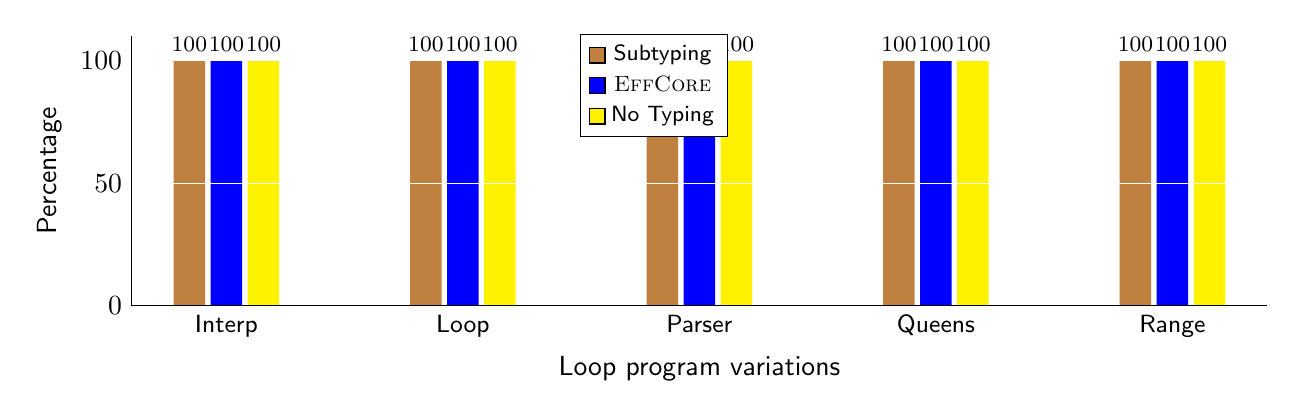
\begin{tikzpicture}
    \centering
    \begin{axis}[
        ybar, axis on top,
        height=5cm, width=16cm,
        ymajorgrids, tick align=inside,
        bar width=0.4cm,
        major grid style={draw=white},
        enlarge y limits={value=.1,upper},
        ymin=0, ymax=100,
        axis x line*=bottom,
        axis y line*=left,
        y axis line style={opacity=1},
        tickwidth=0pt,
        xtick = data,
        x tick label style={font=\small,text width=1.4cm,align=center},
            enlarge x limits=true,
        legend image code/.code={%
        \draw[#1] (0cm,-0.1cm) rectangle (0.2cm,0.1cm);
    },
            legend style={
            at={(0.46,1.01)},
            anchor=north,
            % legend columns=-1,
            % /tikz/every even column/.append style={column sep=0.4cm},
            font = \footnotesize
        },
        ylabel={Percentage},
        xlabel={Loop program variations},
            symbolic x coords={
            Interp,
            Loop,
            Parser,
            Queens,
            Range,
            },
            nodes near coords={
            \footnotesize \pgfmathprintnumber{\pgfplotspointmeta}
        }
    ]
    \addplot [draw=none,fill=brown] coordinates {
        (Interp,100)
        (Loop,100)
        (Parser,100)
        (Queens,100)
        (Range,100)
    };

    \addplot [draw=none,fill=blue] coordinates {
        (Interp,100)
        (Loop,100)
        (Parser,100)
        (Queens,100)
        (Range,100)
    };

    \addplot [draw=none,fill=yellow] coordinates {
        (Interp,100)
        (Loop,100)
        (Parser,100)
        (Queens,100)
        (Range,100)
    };
    
    \legend{Subtyping, \core, No Typing}
    \end{axis}
    \end{tikzpicture}
\caption{Relative run-times of testing programs}
\label{fig:test}
\end{figure}
    
\subsection{Type Inference Comparison}

The main contribution of this thesis is to extend the algebraic subtyping algorithm with algebraic effects and handlers. The goal is to be able to infer types which are shorter, simpler and more human-readable than types inferred by standard subtyping systems. In this evaluation, several small programs were made and its types inferred by the subtyping and the algebraic subtyping system in order to compare both types. 

Considering that the implementation does not yet support the simplification of types, the results are inaccurate. In order to provide a proper evaluation, the types have been manually simplified using the simplification algorithm. All three types are given in order to the current state of the implementation and to be able to evaluate the algebraic subtyping system.


\todo{give the evaluation results}

\begin{figure}[H]
\begin{center}
\begin{framed}
\begin{minipage}[t]{0.95\columnwidth}
    \begin{mathpar}
    \inferrule[Interp]{}{
        \ctxp \prinent x \T [x : \alpha]\alpha
    }

    \inferrule[Loop]{}{
        \ctxp \prinent x \T [x : \alpha]\alpha
    }

    \inferrule[Parser]{}{
        \ctxp \prinent x \T [x : \alpha]\alpha
    }

    \inferrule[Queens]{}{
        \ctxp \prinent x \T [x : \alpha]\alpha
    }

    \inferrule[Range]{}{
        \ctxp \prinent x \T [x : \alpha]\alpha
    }
\end{mathpar}
\end{minipage}
\end{framed}
\end{center}
\caption{Produced types for Subtyping}\label{fig:inferred:sub}
\end{figure}

\begin{figure}[H]
\begin{center}
\begin{framed}
\begin{minipage}[t]{0.95\columnwidth}
    \begin{mathpar}
    \inferrule[Interp]{}{
        \ctxp \prinent x \T [x : \alpha]\alpha
    }

    \inferrule[Loop]{}{
        \ctxp \prinent x \T [x : \alpha]\alpha
    }

    \inferrule[Parser]{}{
        \ctxp \prinent x \T [x : \alpha]\alpha
    }

    \inferrule[Queens]{}{
        \ctxp \prinent x \T [x : \alpha]\alpha
    }

    \inferrule[Range]{}{
        \ctxp \prinent x \T [x : \alpha]\alpha
    }
\end{mathpar}
\end{minipage}
\end{framed}
\end{center}
\caption{Produced types for \core}\label{fig:inferred:core}
\end{figure}

\begin{figure}[H]
\begin{center}
\begin{framed}
\begin{minipage}[t]{0.95\columnwidth}
    \begin{mathpar}
    \inferrule[Interp]{}{
        \ctxp \prinent x \T [x : \alpha]\alpha
    }

    \inferrule[Loop]{}{
        \ctxp \prinent x \T [x : \alpha]\alpha
    }

    \inferrule[Parser]{}{
        \ctxp \prinent x \T [x : \alpha]\alpha
    }

    \inferrule[Queens]{}{
        \ctxp \prinent x \T [x : \alpha]\alpha
    }

    \inferrule[Range]{}{
        \ctxp \prinent x \T [x : \alpha]\alpha
    }
\end{mathpar}
\end{minipage}
\end{framed}
\end{center}
\caption{Produced types for Algebraic Subtyping}\label{fig:inferred:manual}
\end{figure}

\section{Conclusion}

\section{Future Work}
\todo{write future work}

\subsection{Simplification}

\subsection{Biunification with type automata}

\subsection{Optimization}

\section{Conclusion}

\todo{write conclusion}
Briefly recall what the goal of the work was. Summarize what you have done, summarize the results, and present conclusions. Conclusions include a critical assessment: where the original goals reached? Discuss the limitations of your work. Describe how the work could possibly be extended in the future, mitigating limitations or solving remaining problems.



\appendixpage*          % if wanted
\appendix
% \chapter{Appendix A}
% \input{tex/appendix}

\backmatter

% The bibliography comes after the appendices.
% You can replace the standard "abbrv" bibliography style by another one.
\bibliographystyle{abbrv}
\bibliography{bib/main}

\end{document}
